\documentclass{article}

\usepackage{graphics}
\usepackage[vcentering]{geometry}

\geometry{papersize={5in,3.5in}, top=0.2in, bottom=0.2in}

\pagestyle{empty}

\usepackage{tikz}
\usetikzlibrary{
	arrows,shapes,decorations.pathmorphing,backgrounds,positioning,fit,calc,scopes
}


\tikzset{
	auto,
	compartment/.style={
		rectangle, minimum size=9mm, rounded corners=2mm,
		thick, draw=black!15, top color=white,bottom color=black!30
	},
	%
	bigcompartment/.style={
		rectangle, minimum size=20mm, rounded corners=2mm,
		thick, draw=black!30, top color=white,bottom color=black!20
	},
	%
	point/.style={
		circle, inner sep=2pt, fill=black!5
	},
	%
	mytextbox/.style={
		rectangle, text=black!50, thin, 
		draw=white, top color=white,bottom color=white, fill=white
	}
}


\begin{document}

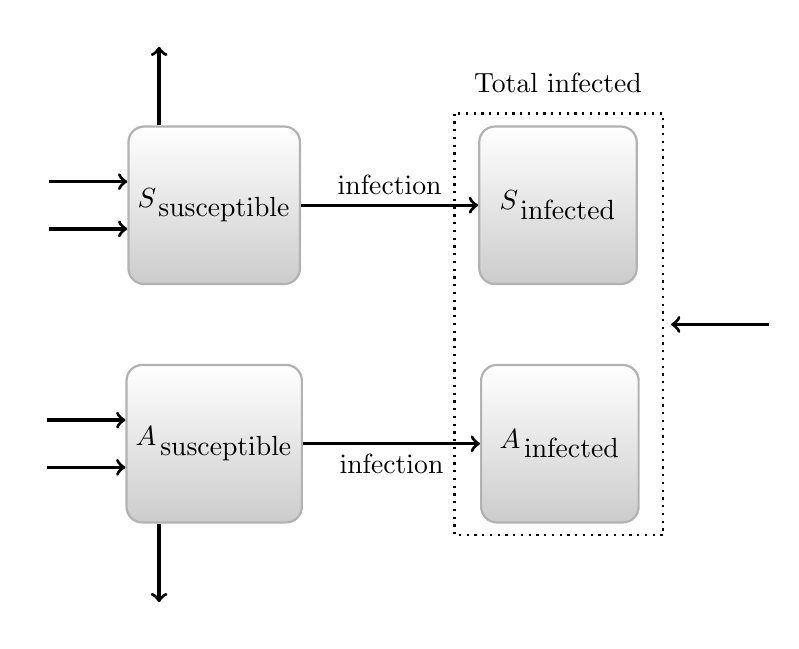
\begin{tikzpicture}
    \node(S)[bigcompartment]{$S_{\,\textrm{susceptible}}$};
    \node(StoSI)[right=of S]{};
    \node(SI)[bigcompartment, right=of StoSI]{$S_{\,\textrm{infected}}$};
    \draw[->, very thick] (S) -- node [text width=2cm, midway, above, align=center] {infection} (SI); 
    \node(A)[bigcompartment, below=of S]{$A_{\,\textrm{susceptible}}$};
    \node(AtoAI)[right=of A]{};
    \node(AI)[bigcompartment, right=of AtoAI]{$A_{\,\textrm{infected}}$};
    \draw[->, very thick] (A) -- node [text width=2cm, midway, below, align=center] {infection} (AI); 
    \node(Sextra)[left=of S]{};
    \draw[->, very thick] ([yshift=0.3 cm]Sextra.east) to ([yshift=0.3 cm]S.west);
    \draw[->, very thick] ([yshift=-0.3 cm]Sextra.east) to ([yshift=-0.3 cm]S.west);
    \node(Sextra2)[above=of S]{};
    \draw[->, very thick] ([xshift=-0.7 cm]S.north) to ([xshift=-0.7 cm]Sextra2.south);
    \node(Aextra)[left=of A]{};
    \draw[->, very thick] ([yshift=0.3 cm]Aextra.east) to ([yshift=0.3 cm]A.west);
    \draw[->, very thick] ([yshift=-0.3 cm]Aextra.east) to ([yshift=-0.3 cm]A.west);
    \node(Aextra2)[below=of A]{};
    \draw[->, very thick] ([xshift=-0.7 cm]A.south) to ([xshift=-0.7 cm]Aextra2.north);
    \draw[thick,dotted] ($(SI.north west)+(-0.3,0.15)$) rectangle ($(AI.south east)+(0.3,-0.15)$);
    \node(I) at ($(AI)!0.5!(SI)$){};
    \node[above] at ([yshift=0.3cm] SI.north){Total infected};
    \node(Iextra)[right=of I]{};
    \draw[->, very thick] ([xshift=1.3cm]Iextra.east) -- ([xshift=1.3cm]I.east);
\end{tikzpicture}

\end{document}
